\documentclass[a4paper,11pt]{article}

\usepackage[utf8]{inputenc}
\usepackage[T1]{fontenc}

\usepackage{makeidx}
\usepackage{color}
\usepackage{graphicx}
\usepackage{float}
\usepackage[hidelinks]{hyperref} 
\usepackage{geometry}
\usepackage{fancyhdr}
\usepackage{amsmath}
\usepackage{empheq}
\usepackage{array}
\usepackage{multicol}
\usepackage{csquotes}
\usepackage{listings}
\usepackage{xcolor}

\definecolor{ligthyellow}{RGB}{250,247,220}
\definecolor{darkblue}{RGB}{5,10,85}
\definecolor{ligthblue}{RGB}{1,147,128}
\definecolor{darkgreen}{RGB}{8,120,51}
\definecolor{darkred}{RGB}{160,0,0}
\definecolor{ivi}{RGB}{141,107,185}


\lstset{
    language = scilab,
    captionpos = b,
    extendedchars = true,
    frame = lines,
    numbers = left,
    numberstyle = \tiny,
    numbersep = 5pt,
    keepspaces = true,
    breaklines = true,
    showspaces = false,
    showstringspaces = false,
    breakatwhitespace = false,
    stepnumber = 1,
    showtabs = false,
    tabsize = 3,
    basicstyle = \small\ttfamily,
    backgroundcolor = \color{ligthyellow},
    keywordstyle = \color{ligthblue},
    morekeywords = {include, printf, uchar},
    identifierstyle = \color{darkblue},
    commentstyle = \color{darkgreen},
    stringstyle = \color{darkred},
}

\setlength{\headheight}{15pt}

\setcounter{secnumdepth}{3}
\setcounter{tocdepth}{2}

\makeatletter
\@addtoreset{chapter}{part}
\makeatother 

\hypersetup{
  colorlinks = true,
  breaklinks = true,
  urlcolor = blue,
  linkcolor = black,
  citecolor = green
}

\title{
  \noindent\hrulefill \\
  \vspace{10mm} Compte-rendu TP1 VisA: Callibration de caméra
}

\title{TP VisA, Algorithmes de type FCM appliqués à l'imagerie couleur}
\author{Tristan Camus et Arnaud Cojez}
\date{}

\definecolor{myColor}{rgb}{0.5, 0.1, 0.75}


\begin{document}


\maketitle

\noindent\hrulefill \\

\section{Introduction}

Poursuivant nos travaux sur la logique floue, nous allons dans ce TP segmenter des images à l'aide de différents algorithmes utilisant de la logique floue.
Alors que l'algorithme du C-Means est déjà fortement utilisé en logique classique, nous allons utiliser différentes variantes de ce dernier utilisant de la logique floue. Nous tenterons ainsi de segmenter, à l'aide des algorithmes Fuzzy C-Means, Hard C-Means, Possibilistic C-Means et de l'algorithme de Davé, l'image suivante en 6 classes distinctes :

\begin{figure}[H]
\begin{center}
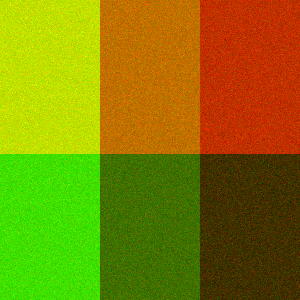
\includegraphics[width=250px]{../img/6_classes_RGB.png}
\end{center}
\caption{Image à segmentée}
\end{figure}

\clearpage

\section{Algorithme FCM}
Fuzzy C-Means est la variante floue la plus simpliste de C-Means. Les résultats de cet algorithme dépandent de la position des centroides calculés aléatoirement au début de l'éxécution. Ainsi, les résultats peuvent varier d'une tentative de classification à une autre. Nous montrons ici des exemples de bonnes classification à l'aide de FCM.

Ainsi, pour les paramètres suivants : 

\begin{table}[H]
  \begin{center}
    \begin{tabular}{|l|c|}
      \hline
      Nombre de classes & 6 \\
      \hline
      Valeur de m & 1 \\
      \hline
      Nombre d'itération & 1000 \\
      \hline
      \shortstack{ Valeur de seuil \\ de stabilité }  & 0.01 \\
      \hline
      Randomisation & 1 \\
      \hline
    \end{tabular}
    \caption{Tableau des paramétres utiliser pour l'algorithme de FCM}
  \end{center}
\end{table}

Nous obtenons l'image suivante :

\begin{figure}[H]
\begin{center}

\includegraphics[width=250px]{../img/FCM.png}
\end{center}
\caption{Image segmentée par FCM}
\end{figure}

Ainsi que la courbe de performance suivante :

\begin{figure}[H]
\begin{center}
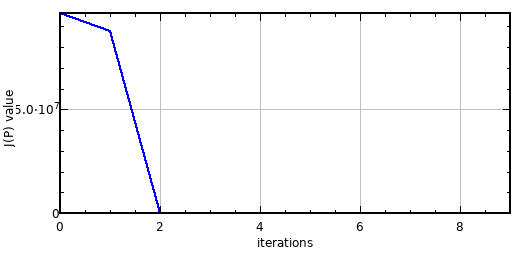
\includegraphics[width=300px]{../img/Perf_FCM.png}
\end{center}
\caption{Courbe de performance pour FCM}
\end{figure}

Le résultat obtenu est assez satisfaisant. On peut distinguer les 6 classes. On note cependant que des points parasites de certaines classes se trouvent dans d'autres.

\section{Algorithme HCM}
Fuzzy C-Means est la variante floue la plus simpliste de C-Means. Les résultats de cet algorithme dépandent de la position des centroides calculés aléatoirement au début de l'éxécution. Ainsi, les résultats peuvent varier d'une tentative de classification à une autre. Nous montrons ici des exemples de bonnes classification à l'aide de HCM.

Ainsi, pour les paramètres suivants : 

\begin{table}[H]
  \begin{center}
    \begin{tabular}{|l|c|}
      \hline
      Nombre de classes & 6 \\
      \hline
      Valeur de m & 1 \\
      \hline
      Nombre d'itération & 1000 \\
      \hline
      \shortstack{ Valeur de seuil \\ de stabilité }  & 0.01 \\
      \hline
      Randomisation & 1 \\
      \hline
    \end{tabular}
    \caption{Tableau des paramétres utiliser pour l'algorithme de HCM}
  \end{center}
\end{table}

Nous obtenons l'image suivante :

\begin{figure}[H]
\begin{center}
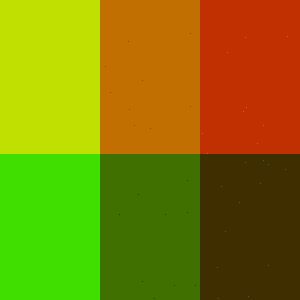
\includegraphics[width=250px]{../img/HCM.png}
\end{center}
\caption{Image segmentée par HCM}
\end{figure}

Ainsi que la courbe de performance suivante :

\begin{figure}[H]
\begin{center}
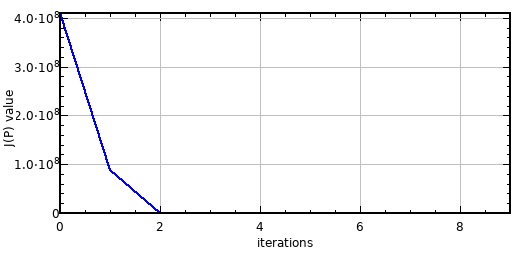
\includegraphics[width=300px]{../img/Perf_HCM.png}
\end{center}
\caption{Courbe de performance pour HCM}
\end{figure}

Le résultat obtenu est assez satisfaisant. On peut distinguer les 6 classes. On note cependant que des points parasites de certaines classes se trouvent dans d'autres.

\section{Algorithme PCM}
Fuzzy C-Means est la variante floue la plus simpliste de C-Means. Les résultats de cet algorithme dépandent de la position des centroides calculés aléatoirement au début de l'éxécution. Ainsi, les résultats peuvent varier d'une tentative de classification à une autre. Nous montrons ici des exemples de bonnes classification à l'aide de PCM.

Ainsi, pour les paramètres suivants : 

\begin{table}[H]
  \begin{center}
    \begin{tabular}{|l|c|}
      \hline
      Nombre de classes & 6 \\
      \hline
      Valeur de m & 1 \\
      \hline
      Nombre d'itération & 1000 \\
      \hline
      \shortstack{ Valeur de seuil \\ de stabilité }  & 0.01 \\
      \hline
      Randomisation & 1 \\
      \hline
    \end{tabular}
    \caption{Tableau des paramétres utiliser pour l'algorithme de PCM}
  \end{center}
\end{table}

Nous obtenons l'image suivante :

\begin{figure}[H]
\begin{center}

\includegraphics[width=250px]{../img/PCM.png}
\end{center}
\caption{Image segmentée par PCM}
\end{figure}

Ainsi que la courbe de performance suivante :

\begin{figure}[H]
\begin{center}
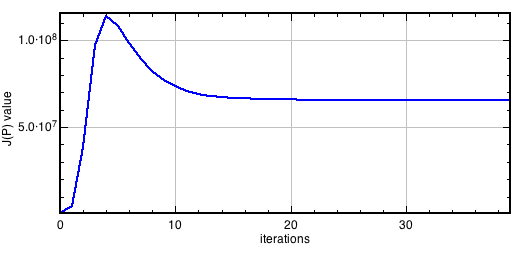
\includegraphics[width=300px]{../img/Perf_PCM.png}
\end{center}
\caption{Courbe de performance pour PCM}
\end{figure}

Le résultat obtenu est assez satisfaisant. On peut distinguer les 6 classes. On note cependant que des points parasites de certaines classes se trouvent dans d'autres.

\section{Algorithme de Davé}
Fuzzy C-Means est la variante floue la plus simpliste de C-Means. Les résultats de cet algorithme dépandent de la position des centroides calculés aléatoirement au début de l'éxécution. Ainsi, les résultats peuvent varier d'une tentative de classification à une autre. Nous montrons ici des exemples de bonnes classification à l'aide de FCM.

Ainsi, pour les paramètres suivants : 

\begin{table}[H]
  \begin{center}
    \begin{tabular}{|l|c|}
      \hline
      Nombre de classes & 6 \\
      \hline
      Valeur de m & 1 \\
      \hline
      Nombre d'itération & 1000 \\
      \hline
      \shortstack{ Valeur de seuil \\ de stabilité }  & 0.01 \\
      \hline
      Randomisation & 1 \\
      \hline
    \end{tabular}
    \caption{Tableau des paramétres utiliser pour l'algorithme de Davé}
  \end{center}
\end{table}

Nous obtenons l'image suivante :

\begin{figure}[H]
\begin{center}
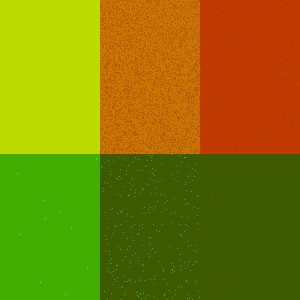
\includegraphics[width=250px]{../img/Dave.png}
\end{center}
\caption{Image segmentée par l'algorithme de Davé}
\end{figure}

Ainsi que la courbe de performance suivante :

\begin{figure}[H]
\begin{center}
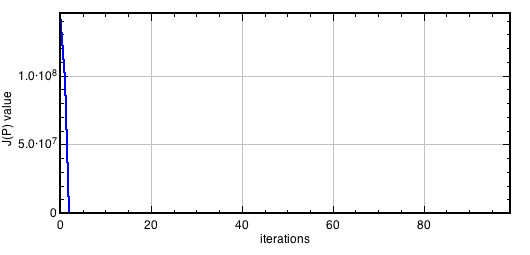
\includegraphics[width=300px]{../img/Perf_Dave.png}
\end{center}
\caption{Courbe de performance pour l'algorithme de Davé}
\end{figure}

Le résultat obtenu est assez satisfaisant. On peut distinguer les 6 classes. On note cependant que des points parasites de certaines classes se trouvent dans d'autres.

\clearpage

\section{Conclusion}
Nous pouvons conclure que les différentes méthodes vues lors de ces TPs, 
ne sont pas véritablement des algorithmes de segmentations. En effet, 
elles calculent des degrés d'appartenance qui ne permettent pas de 
segmenter directement les images.\\

Pour segmenter les images dont les degrés d'appartenance aux classes ont 
été calculés, il faut définir des heuristiques qui vont séparer les 
pixels.\\

Il sagit pas d'une vraie segmentation


\end{document}